\section{NHIỆT NÓNG CHẢY RIÊNG - NHIỆT HOÁ HƠI RIÊNG}
\subsection{LÝ THUYẾT TRỌNG TÂM}
\begin{tomtat}
	\subsubsection{Nhiệt nóng chảy riêng}
	\begin{dn}
		Nhiệt nóng chảy riêng của một chất rắn có giá trị bằng nhiệt lượng cần cung cấp cho $\SI{1}{\kilogram}$ chất đó chuyển từ thể rắn sang thể lỏng tại nhiệt độ nóng chảy:
		\begin{equation}
			\lambda=\dfrac{Q}{m}
		\end{equation}
	\end{dn}
	với
	\begin{itemize}
		\item $\lambda$: nhiệt nóng chảy riêng, đơn vị trong hệ SI là $\si{\joule/\kilogram}$;
		\item $Q$: nhiệt lượng khối chất rắn thu vào để nóng chảy hoàn toàn, đơn vị trong hệ SI là $\si{\joule}$;
		\item $m$: khối lượng của khối chất rắn, đơn vị trong hệ SI là $\si{\kilogram}$.
	\end{itemize}
	\subsubsection{Nhiệt hoá hơi riêng}
	\begin{dn}
		Nhiệt hoá hơi riêng của một chất lỏng có giá trị bằng nhiệt lượng cần cung cấp cho $\SI{1}{\kilogram}$ chất lỏng đó hoá hơi hoàn toàn ở nhiệt độ sôi:
		\begin{equation}
			L=\dfrac{Q}{m}
		\end{equation}
	\end{dn}
	với
	\begin{itemize}
		\item $L$: nhiệt hoá hơi riêng, đơn vị trong hệ SI là $\si{\joule/\kilogram}$;
		\item $Q$: nhiệt lượng khối chất lỏng thu vào để hoá hơi hoàn toàn, đơn vị trong hệ SI là $\si{\joule}$;
		\item $m$: khối lượng của khối chất lỏng, đơn vị trong hệ SI là $\si{\kilogram}$.
	\end{itemize}
\end{tomtat}
\subsection{VÍ DỤ MINH HOẠ}
\begin{dang}{Vận dụng biểu thức xác định nhiệt nóng chảy riêng}
\end{dang}
\begin{vd}
Một nhà máy thép mỗi lần luyện được 35 tấn thép. Cho nhiệt nóng chảy riêng của thép là $\SI{2.77E5}{\joule/\kilogram}$.
		\begin{enumerate}[label=\alph*)]
			\item Tính nhiệt lượng cần cung cấp để làm nóng chảy thép trong mỗi lần luyện của nhà máy ở nhiệt độ nóng chảy.
			\item Giả sử nhà máy sử dụng khí đốt để nấu chảy thép trong lò thổi (nồi nấu thép). Biết khi đốt cháy hoàn toàn $\SI{1}{\kilogram}$ khí đốt thì nhiệt lượng toả ra là $\SI{44E6}{\joule}$. Xác định khối lượng khí đốt cần sử dụng.
		\end{enumerate}

	\loigiai{
			\begin{enumerate}[label=\alph*)]
				\item Nhiệt lượng cần cung cấp để làm nóng chảy thép trong mỗi lần luyện của nhà máy ở nhiệt độ nóng chảy:
				$$Q=m\lambda=\left(\SI{35E3}{\kilogram}\right)\cdot\left(\SI{2.77E5}{\joule/\kilogram}\right)=\SI{96.95E8}{\joule}$$
				\item Khối lượng khí đốt cần sử dụng để nhiệt lượng toả ra như ở câu a):
				$$m=\dfrac{Q}{q}=\dfrac{\SI{96.95E8}{\joule}}{\SI{44E6}{\joule/\kilogram}}\approx\SI{220.34}{\kilogram}$$
		\end{enumerate}}
\end{vd}
	
	\begin{vd}
		Tính thời gian cần thiết để làm nóng chảy hoàn toàn $\SI{2}{\kilogram}$ đồng có nhiệt độ ban đầu $\SI{30}{\celsius}$, trong một lò nung điện có công suất $\SI{20000}{\watt}$. Biết chỉ có $\SI{50}{\percent}$ năng lượng tiêu thụ của lò được dùng vào việc làm đồng nóng lên và nóng chảy hoàn toàn ở nhiệt độ không đổi. Biết nhiệt độ nóng chảy của đồng là $\SI{1084}{\celsius}$. Cho nhiệt dung riêng, nhiệt nóng chảy riêng của đồng lần lượt là $\SI{380}{\joule/\left(\kilogram\cdot\kelvin\right)}$ và $\SI{1.8E5}{\joule/\kilogram}$.
	\loigiai{
				Nhiệt lượng khối đồng cần thu vào để tăng nhiệt độ từ $\SI{30}{\celsius}$ đến $\SI{1084}{\celsius}$:
				$$Q_1=mc\Delta t=\left(\SI{2}{\kilogram}\right)\cdot\left[\SI{380}{\joule/\left(\kilogram\cdot\kelvin\right)}\right]\cdot\left(\SI{1084}{\celsius}-\SI{30}{\celsius}\right)=\SI{801.04}{\kilo\joule}$$
				Nhiệt lượng khối đồng cần thu vào để nóng chảy hoàn toàn ở nhiệt độ $\SI{1084}{\celsius}$:
				$$Q_2=m\lambda=\left(\SI{2}{\kilogram}\right)\cdot\left(\SI{1.8E5}{\joule/\kilogram}\right)=\SI{360}{\kilo\joule}$$
				Tổng nhiệt lượng $\SI{2}{\kilogram}$ đồng cần thu vào để nóng chảy hoàn toàn từ nhiệt độ ban đầu $\SI{30}{\celsius}$:
				$$Q=Q_1+Q_2=\SI{1161.04}{\kilo\joule}$$
				Thời gian cần thiết để làm nóng chảy hoàn toàn khối đồng này:
				$$t=\dfrac{Q}{H\cdot\calP}=\dfrac{\SI{1161.04E3}{\joule}}{\left(\SI{50}{\percent}\right)\cdot\left(\SI{2E4}{\watt}\right)}\approx\SI{116}{\second}$$
			}
	\end{vd}
	
	\begin{dang}{Vận dụng biểu thức xác định nhiệt hoá hơi riêng}
			\end{dang}
\begin{vd}
Tính nhiệt lượng cần thiết để làm cho $\SI{1}{\kilogram}$ nước ở $\SI{25}{\celsius}$ chuyển thành hơi ở $\SI{100}{\celsius}$. Cho nhiệt dung riêng của nước là $\SI{4200}{\joule/\left(\kilogram\cdot\kelvin\right)}$, nhiệt hoá hơi riêng của nước ở $\SI{100}{\celsius}$ là $\SI{2.26E6}{\joule/\kilogram}$.
\loigiai{
		Nhiệt lượng nước thu vào để tăng nhiệt độ từ $\SI{25}{\celsius}$ đến $\SI{100}{\celsius}$:
		$$Q_1=mc\Delta t=\left(\SI{1}{\kilogram}\right)\cdot\left[\SI{4200}{\joule/\left(\kilogram\cdot\kelvin\right)}\right]\cdot\left(\SI{100}{\celsius}-\SI{25}{\celsius}\right)=\SI{315E3}{\joule}$$
		Nhiệt lượng nước cần thu vào để hoá thành hơi hoàn toàn ở $\SI{100}{\celsius}$:
		$$Q_2=mL=\left(\SI{1}{\kilogram}\right)\cdot\left(\SI{2.26E6}{\joule/\kilogram}\right)=\SI{226E4}{\joule}$$
		Tổng nhiệt lượng nước cần thu vào để hoá hơi hoàn toàn ở $\SI{100}{\celsius}$:
		$$Q=Q_1+Q_2=\SI{2.575}{\mega\joule}$$
	}

\end{vd}
		
		\begin{vd}
			Một ấm đun nước có công suất $\SI{500}{\watt}$ chứa $\SI{300}{\gram}$ nước ở nhiệt độ $\SI{20}{\celsius}$. Cho nhiệt dung riêng của nước là $\SI{4200}{\joule/\left(\kilogram\cdot\kelvin\right)}$, nhiệt hoá hơi riêng của nước ở $\SI{100}{\celsius}$ là $\SI{2.26E6}{\joule/\kilogram}$.
				\begin{enumerate}[label=\alph*)]
					\item Tính thời gian cần thiết để đun nước trong ấm để đạt đến nhiệt độ sôi.
					\item Sau khi nước đến nhiệt độ sôi, người ta để ấm tiếp tục đun nước sôi trong 2 phút. Tính khối lượng nước còn lại trong ấm và chỉ rõ điều kiện để thực hiện các tính toán đó.
				\end{enumerate}
			\loigiai{
					\begin{enumerate}[label=\alph*)]
						\item Nhiệt lượng nước trong ấm cần thu vào để tăng nhiệt độ từ $\SI{20}{\celsius}$ đến nhiệt độ sôi $\left(\SI{100}{\celsius}\right)$:
						$$Q_1=mc\Delta t=\left(\SI{0.3}{\kilogram}\right)\cdot\left[\SI{4200}{\joule/\left(\kilogram\cdot\kelvin\right)}\right]\cdot\left(\SI{100}{\celsius}-\SI{20}{\celsius}\right)=\SI{100800}{\joule}$$
						Thời gian đun sôi nước:
						$$t=\dfrac{Q_1}{\calP}=\dfrac{\SI{100800}{\joule}}{\SI{500}{\watt}}\approx\SI{201}{\second}$$
						\item Nhiệt lượng ấm toả ra trong 2 phút:
						$$Q_2=\calP\cdot t'=\left(\SI{500}{\watt}\right)\cdot\left(\SI{120}{\second}\right)=\SI{60}{\kilo\joule}$$
						Khối lượng nước bị hoá thành hơi ở nhiệt độ $\SI{100}{\celsius}$:
						$$m'=\dfrac{Q_2}{L}=\dfrac{\SI{60E3}{\joule}}{\SI{2.26E6}{\joule/\kilogram}}\approx\SI{26.55}{\gram}$$
						Khối lượng nước còn lại trong ấm:
						$$m_\text{nước}=m-m'=\SI{273.45}{\gram}$$
						Các tính toán trên được thực hiện với điều kiện:
						\begin{itemize}
							\item Nước được đun ở áp suất $\SI{1}{atm}$, do đó nhiệt độ sôi của nước là $\SI{100}{\celsius}$.
							\item Bỏ qua nhiệt lượng cung cấp cho vỏ ấm đun và toả ra môi trường.
							\item Bỏ qua sự bay hơi của nước trong quá trình đun.
						\end{itemize}
					\end{enumerate}
				}
		\end{vd}
	\begin{dang}{Bài toán về hiệu suất truyền nhiệt}
	\end{dang}
	\begin{vd}
		Dùng bếp điện để đun một ấm nhôm khối lượng $\SI{600}{\gram}$ đựng 1,5 lít nước ở nhiệt độ $\SI{20}{\celsius}$. Sau 35 phút đã có $\SI{20}{\percent}$ lượng nước trong ấm hoá hơi ở nhiệt độ $\SI{100}{\celsius}$. Tính nhiệt lượng trung bình mà bếp điện cung cấp cho ấm nước trong mỗi giây, biết chỉ có $\SI{75}{\percent}$ nhiệt lượng mà bếp toả ra được dùng vào việc đun ấm nước. Biết nhiệt dung riêng của nhôm là $\SI{880}{\joule/\left(\kilogram\cdot\kelvin\right)}$, của nước là $\SI{4190}{\joule/\left(\kilogram\cdot\kelvin\right)}$; nhiệt hoá hơi riêng của nước ở nhiệt độ sôi $\SI{100}{\celsius}$ là $\SI{2.26E6}{\joule/\kilogram}$, khối lượng riêng của nước là $\SI{1}{\kilogram/\text{lít}}$.
		\loigiai{Gọi:
			\begin{itemize}
				\item $m_1$, $c_1$ lần lượt là khối lượng ấm nhôm và nhiệt dung riêng của nhôm;
				\item $m_2$, $c_2$ lần lượt là khối lượng của nước và nhiệt dung riêng của nước.
			\end{itemize}
			Khối lượng nước trong ấm:
			$$m_2=V_2D_2=\left(\SI{1.5}{\text{lít}}\right)\cdot\left(\SI{1.5}{\kilogram/\text{lít}}\right)=\SI{1.5}{\kilogram}.$$
			Nhiệt lượng ấm nhôm thu vào để tăng nhiệt độ từ $\SI{20}{\celsius}$ lên $\SI{100}{\celsius}$:
			$$Q_1=m_1c_1\Delta t=\left(\SI{0.6}{\kilogram}\right)\cdot\left[\SI{880}{\joule/\left(\kilogram\cdot\kelvin\right)}\right]\cdot\left(\SI{100}{\celsius}-\SI{20}{\celsius}\right)=\SI{42240}{\joule}.$$
			Nhiệt lượng nước thu vào để tăng nhiệt độ từ $\SI{20}{\celsius}$ lên $\SI{100}{\celsius}$ và $\SI{20}{\percent}$ lượng nước hoá thành hơi:
			$$Q_2=m_2c_2\Delta t+\SI{20}{\percent}m_2L=\left(\SI{1.5}{\kilogram}\right)\cdot\left[\SI{4190}{\joule/\left(\kilogram\cdot\kelvin\right)}\right]\cdot\left(\SI{80}{\celsius}\right)+\SI{20}{\percent}\cdot\left(\SI{1.5}{\kilogram}\right)\cdot\left(\SI{2.26E6}{\joule/\kilogram}\right)=\SI{1180.8}{\kilo\joule}.$$
			Nhiệt lượng do bếp điện cung cấp:
			$$Q=\dfrac{Q_1+Q_2}{H}=\SI{1630.72}{\kilo\joule}.$$
			Nhiệt lượng trung bình mà bếp điện cung cấp cho ấm nước trong mỗi giây:
			$$\calP=\dfrac{Q}{t}=\dfrac{\SI{1630.72}{\kilo\joule}}{35\cdot\SI{60}{\second}}\approx\SI{776.5}{\watt}.$$
		}
		
	\end{vd}
	
	% ========================================
	\begin{vd}
		\begin{enumerate}[label=\alph*)]
			\item Tính nhiệt lượng cần thiết để $\SI{2}{\kilogram}$ nước đá ở $\SI{-10}{\celsius}$ hoá hơi hoàn toàn ở nhiệt độ sôi, cho biết:
			\begin{itemize}
				\item nhiệt dung riêng của nước đá là $\SI{1800}{\joule/\left(\kilogram\cdot\kelvin\right)}$;
				\item nhiệt dung riêng của nước $\SI{4200}{\joule/\left(\kilogram\cdot\kelvin\right)}$;
				\item nhiệt nóng chảy riêng của nước đá là $\SI{34E4}{\joule/\kilogram}$;
				\item nhiệt hoá hơi riêng của nước là $\SI{23E5}{\joule/\kilogram}$.
			\end{itemize}
			\item Nếu dùng một bếp dầu hoả có hiệu suất $\SI{80}{\percent}$, người ta phải đốt cháy hoàn toàn bao nhiêu lít dầu để cho $\SI{2}{\kilogram}$ nước đá ở $\SI{-10}{\celsius}$ biến thành hơi.\\
			Cho biết:
			\begin{itemize}
				\item khối lượng riêng của dầu hoả là $\SI{800}{\kilogram/\meter^3}$;
				\item năng suất toả nhiệt của dầu hoả là $\SI{44E6}{\joule/\kilogram}$.
			\end{itemize}
		\end{enumerate}
		\loigiai{\begin{enumerate}[label=\alph*)]
				\item Quá trình nước đá $\SI{-10}{\celsius}$ hoá hơi hoàn toàn ở nhiệt độ sôi trải qua 4 giai đoạn:
				\begin{itemize}
					\item Nước đá thu nhiệt để tăng nhiệt độ từ $\SI{-10}{\celsius}$ lên $\SI{0}{\celsius}$: 
					$$Q_1=mc_\text{đ}\left(0-t_0\right)=\left(\SI{2}{\kilogram}\right)\cdot\left[\SI{1800}{\joule/\left(\kilogram\cdot\kelvin\right)}\right]\cdot\left(\SI{10}{\celsius}\right)=\SI{36}{\kilo\joule}.$$
					\item Nước đá thu nhiệt để nóng chảy hoàn toàn ở $\SI{0}{\celsius}$:
					$$Q_2=m\lambda=\left(\SI{2}{\kilogram}\right)\cdot\left(\SI{34E4}{\joule/\kilogram}\right)=\SI{680}{\kilo\joule}.$$
					\item Nước thu nhiệt để tăng nhiệt độ từ $\SI{0}{\celsius}$ đến $\SI{100}{\celsius}$:
					$$Q_3=mc_\text{n}\left(\SI{100}{\celsius}-\SI{0}{\celsius}\right)=\left(\SI{2}{\kilogram}\right)\cdot\left[\SI{4200}{\joule/\left(\kilogram\cdot\kelvin\right)}\right]\cdot\left(\SI{100}{\celsius}\right)=\SI{840}{\kilo\joule}.$$
					\item Nước hoá hơi hoàn toàn ở $\SI{100}{\celsius}$:
					$$Q_4=mL=\left(\SI{2}{\kilogram}\right)\cdot\left(\SI{23E5}{\joule/\kilogram}\right)=\SI{4600}{\kilo\joule}.$$
				\end{itemize}
				Tổng nhiệt lượng đá cần thu vào để hoá hơi hoàn toàn ở $\SI{100}{\celsius}$:
				$$Q=Q_1+Q_2+Q_3+Q_4=\SI{6156}{\kilo\joule}.$$
				\item Nhiệt lượng bếp dầu cần cung cấp:
				$$Q_\text{tp}=\dfrac{Q}{H}=\dfrac{\SI{6156}{\kilo\joule}}{\SI{80}{\percent}}=\SI{7695}{\kilo\joule}.$$
				Khối lượng dầu cần đốt để tạo ra nhiệt lượng như trên:
				$$m=\dfrac{Q_\text{tp}}{q}=\dfrac{\SI{7695E3}{\joule}}{\SI{44E6}{\joule/\kilogram}}\approx\SI{0.175}{\kilogram}.$$
				Thể tích dầu cần đốt:
				$$V=\dfrac{m}{D}=\dfrac{\SI{0.175}{\kilogram}}{\SI{800}{\kilogram/\meter^3}}\approx\SI{2.19E-4}{\meter^3}=\SI{0.219}{\text{lít}}.$$
			\end{enumerate}
		}
		
	\end{vd}
	\begin{dang}
		{Áp dụng phương trình cân bằng nhiệt khi có sự chuyển thể}
		\begin{center}
			\includegraphics[width=0.8\linewidth]{figs/VN12-Y24-PH-SYL-006-1}
			\captionof{figure}{Sơ đồ chuyển thể}
		\end{center}
	\end{dang}
\begin{vd}
	Rót nước ở nhiệt độ $t_1=\SI{20}{\celsius}$ vào một nhiệt lượng kế. Thả vào trong nhiệt lượng kế một cục nước đá khối lượng $m_2=\SI{0.5}{\kilogram}$ và nhiệt độ $t_2=\SI{-15}{\celsius}$. Biết khối lượng nước đổ vào $m_1=m_2$. Cho biết nhiệt dung riêng của nước $c_1=\SI{4200}{\joule/\left(\kilogram\cdot\kelvin\right)}$, của nước đá $c_2=\SI{2100}{\joule/\left(\kilogram\cdot\kelvin\right)}$ và nhiệt nóng chảy riêng của nước đá $\lambda=\SI{3.4E5}{\joule/\kilogram}$. Bỏ qua sự trao đổi nhiệt với môi trường.
	\begin{enumerate}[label=\alph*)]
		\item Hãy cho biết cục nước đá có tan hết không?
		\item Nếu nước đá tan hết, hãy xác định nhiệt độ của hỗn hợp sau khi cân bằng nhiệt được thiết lập. Nếu nước đá không tan hết, hãy tính khối lượng nước đá đã tan.
	\end{enumerate}
\loigiai{
\begin{enumerate}[label=\alph*)]
	\item Nhiệt lượng nước $\SI{20}{\celsius}$ toả ra để giảm nhiệt độ xuống $\SI{0}{\celsius}$:
	$$Q_1=m_1c_1\left(0-t_1\right)=\left(\SI{0.5}{\kilogram}\right)\cdot\left[\SI{4200}{\joule/\left(\kilogram\cdot\kelvin\right)}\right]\cdot\left(\SI{0}{\celsius}-\SI{20}{\celsius}\right)=\SI{-42000}{\joule}$$
	Nhiệt lượng nước đá cần thu vào để tăng nhiệt độ từ $\SI{-15}{\celsius}$ đến $\SI{0}{\celsius}$ và nóng chảy hoàn toàn:
	$$Q_2=m_2c_2\left(0-t_2\right)+m_2\lambda$$
	$$\Leftrightarrow Q_2=\left(\SI{0.5}{\kilogram}\right)\cdot\left[\SI{2100}{\joule/\left(\kilogram\cdot\kelvin\right)}\right]\cdot\left(\SI{0}{\celsius}+\SI{15}{\celsius}\right)+\left(\SI{0.5}{\kilogram}\right)\cdot\left(\SI{3.4E5}{\joule/\kilogram}\right)=\SI{185750}{\joule}$$
	Vì $\left|Q_1\right|<Q_2$ nên nước đá chỉ tan được một phần.
	\item Vì nước đá chỉ tan một phần nên nhiệt độ của hỗn hợp khi cân bằng nhiệt là $\SI{0}{\celsius}$.\\
	Gọi $m'$ là khối lượng nước đá đã tan.\\
	Nhiệt lượng nước đá cần thu vào để tăng nhiệt độ từ $\SI{-15}{\celsius}$ đến $\SI{0}{\celsius}$ và nóng chảy một phần: $$Q_2'=m_2c_2\left(0-t_2\right)+m'\lambda$$
	Trạng thái cân bằng nhiệt được thiết lập khi tổng nhiệt lượng trao đổi trong hệ bằng 0:
	$$Q_1+Q_2'=0$$
	$$\Leftrightarrow Q_1+m_2c_2\left(0-t_2\right)+m'\lambda=0$$
	\begin{eqnarray*}
		\Rightarrow m'&=&-\dfrac{Q_1+m_2c_2\left(0-t_2\right)}{\lambda}\\
		\Leftrightarrow m'&=&-\dfrac{\SI{-42000}{\joule}+\left(\SI{0.5}{\kilogram}\right)\cdot\left[\SI{2100}{\joule/\left(\kilogram\cdot\kelvin\right)}\right]\cdot\left(\SI{0}{\celsius}+\SI{15}{\celsius}\right)}{\SI{3.4E5}{\joule/\kilogram}}\\
		\Rightarrow m'&\approx&\SI{77.2}{\gram}.
	\end{eqnarray*}
	Vậy khối lượng nước đá đã tan là $\SI{77.2}{\gram}$.
	
	
\end{enumerate}
}
\end{vd}
% ========================================================================
\begin{vd}
	Dẫn $m_1=\SI{100}{\gram}$ hơi nước ở $t_1=\SI{100}{\celsius}$ vào một bình cách nhiệt đựng nước đá ở $t_2=\SI{-4}{\celsius}$. Nước đá bị tan hoàn toàn và nhiệt độ nước trong bình sau khi cân bằng nhiệt là $\SI{10}{\celsius}$. Tìm khối lượng nước đá trong bình. Biết nhiệt nóng chảy riêng của nước đá là $\lambda=\SI{3.4E5}{\joule/\kilogram}$, nhiệt hoá hơi riêng của nước ở $\SI{100}{\celsius}$ là $L=\SI{2.3E6}{\joule/\kilogram}$, nhiệt dung riêng của nước là $c_1=\SI{4200}{\joule/\left(\kilogram\cdot\kelvin\right)}$, nhiệt dung riêng của nước đá là $c_2=\SI{2100}{\joule/\left(\kilogram\cdot\kelvin\right)}$. Bỏ qua sự trao đổi nhiệt với môi trường.
	\loigiai{
	Gọi $\xsi{m}{\left(\kilogram\right)}$ là khối lượng nước đá trong bình.\\
	Nhiệt lượng hơi nước toả ra để ngưng tụ hoàn toàn ở $\SI{100}{\celsius}$ và giảm nhiệt độ từ $\SI{100}{\celsius}$ xuống $\SI{10}{\celsius}$:
	$$Q_1=-m_1L+m_1c_1\left(t_\text{cb}-t_1\right)$$
	$$\Leftrightarrow Q_1=-\left(\SI{0.1}{\kilogram}\right)\cdot\left(\SI{2.3E6}{\joule/\kilogram}\right)+\left(\SI{0.1}{\kilogram}\right)\cdot\left[\SI{4200}{\joule/\left(\kilogram\cdot\kelvin\right)}\right]\cdot\left(\SI{10}{\celsius}-\SI{100}{\celsius}\right)=\SI{-267800}{\joule}$$
	Nhiệt lượng nước đá thu vào để tăng nhiệt độ từ $\SI{-4}{\celsius}$ lên $\SI{0}{\celsius}$, nóng chảy hoàn toàn ở $\SI{0}{\celsius}$ rồi tăng nhiệt độ lên $\SI{10}{\celsius}$:
	$$Q_2=mc_2\left(0-t_2\right)+m\lambda+mc_1\left(t_\text{cb}-0\right)$$
	$$\Leftrightarrow Q_2=m\cdot\left[\SI{2100}{\joule/\left(\kilogram\cdot\kelvin\right)}\right]\cdot\left(\SI{0}{\celsius}+\SI{4}{\celsius}\right)+m\cdot\left(\SI{3.4E5}{\joule/\kilogram}\right)+m\cdot\left[\SI{4200}{\joule/\left(\joule\cdot\kelvin\right)}\right]\cdot\left(\SI{10}{\celsius}-\SI{0}{\celsius}\right)=390400m$$
	Hệ đạt trạng thái cân bằng nhiệt khi tổng nhiệt lượng trao đổi trong hệ bằng 0:
	\begin{eqnarray*}
		&&Q_1+Q_2=0\\
		&\Leftrightarrow& -267800+390400m=0\\
		&\Rightarrow& m\approx\SI{0.686}{\kilogram}.
	\end{eqnarray*}
}
\end{vd}
\subsection{BÀI TẬP TRẮC NGHIỆM}
\setcounter{ex}{0}
\Opensolutionfile{ans}[ans/G12Y24B6TN]		
% ===================================================================
\begin{ex}
Khi vật rắn tinh thể đang nóng chảy thì đại lượng nào của vật sau đây là không thay đổi?	
\choice
{Thể tích}
{Nội năng}
{\True Nhiệt độ}
{Hình dạng}
\loigiai{}
\end{ex}
% ===================================================================
\begin{ex}
	Điều nào sau đây là \textbf{đúng} khi nói về nhiệt nóng chảy riêng?
	\choice
	{Nhiệt nóng chảy riêng của chất rắn là nhiệt lượng cần cung cấp cho vật rắn trong quá trình nóng chảy}
	{Các chất có khối lượng bằng nhau thì có nhiệt độ nóng chảy như nhau}
	{Nhiệt nóng chảy riêng của chất rắn tỉ lệ thuận với khối lượng của vật}
	{\True Đơn vị của nhiệt nóng chảy riêng là $\si{\joule/\kilogram}$}
	\loigiai{}
\end{ex}
% ===================================================================
\begin{ex}
	Nhiệt nóng chảy riêng của đồng là $\SI{1.8E5}{\joule/\kilogram}$. Câu nào dưới đây là \textbf{đúng}?
	\choice
	{Khối đồng sẽ toả ra nhiệt lượng $\SI{1.8E5}{\joule}$ khi nóng chảy hoàn toàn}
	{\True Mỗi kilogram đồng cần thu nhiệt lượng $\SI{1.8E5}{\joule}$ để hoá lỏng hoàn toàn ở nhiệt độ nóng chảy}
	{Khối đồng cần nhu nhiệt lượng $\SI{1.8E5}{\joule}$ để hoá lỏng}
	{Mỗi kilogram đồng toả ra nhiệt lượng $\SI{1.8E5}{\joule}$ khi hoá lỏng hoàn toàn}
	\loigiai{}
\end{ex}
% ===================================================================
\begin{ex}
	Đơn vị của nhiệt hoá hơi riêng của chất lỏng là
	\choice
	{\True $\si{\joule/\kilogram}$}
	{$\si{\joule\cdot\kilogram}$}
	{$\si{\kilogram/\joule}$}
	{$\si{\joule}$}
	\loigiai{}
\end{ex}
% ===================================================================
\begin{ex}
	Nhiệt hoá hơi riêng của nước là $\SI{2.3E6}{\joule/\kilogram}$. Câu nào dưới đây là \textbf{đúng nhất}?
	\choice
	{Mỗi lượng nước bất kì cần thu một lượng nhiệt $\SI{2.3E6}{\joule}$ để bay hơi hoàn toàn}
	{Mỗi kilogram nước cần thu một lượng nhiệt là $\SI{2.3E6}{\joule}$ để bay hơi hoàn toàn}
	{Mỗi kilogram nước sẽ toả ra một lượng nhiệt là $\SI{2.3E6}{\joule}$ khi bay hơi hoàn toàn ở nhiệt độ sôi}
	{\True Mỗi kilogram nước cần thu một lượng nhiệt là $\SI{2.3E6}{\joule}$ để bay hơi hoàn toàn ở nhiệt độ sôi và áp suất chuẩn}
	\loigiai{}
\end{ex}
% ===================================================================
\begin{ex}
	Biết nhiệt nóng chảy riêng của nước đá là $\SI{3.34E5}{\joule/\kilogram}$. Nhiệt lượng cần cung cấp để làm nóng chảy $\SI{500}{\gram}$ nước đá ở $\SI{0}{\celsius}$ là
	\choice
	{$\SI{7E7}{\joule}$}
	{$\SI{167}{\joule}$}
	{\True $\SI{167}{\kilo\joule}$}
	{$\SI{167e6}{\joule}$}
	\loigiai{	$$Q=m\lambda=\left(\SI{0.5}{\kilogram}\right)\cdot\left(\SI{3.34E5}{\joule/\kilogram}\right)=\SI{167}{\kilo\joule}$$}
\end{ex}
% ===================================================================
\begin{ex}
	Biết nhiệt dung riêng của nước là $c=\SI{4190}{\joule/\left(\kilogram\cdot\kelvin\right)}$ và nhiệt hoá hơi riêng của nước là $L=\SI{2.26E6}{\joule/\kilogram}$. Để làm cho $\SI{200}{\gram}$ nước ở $\SI{10}{\celsius}$ sôi ở $\SI{100}{\celsius}$ và $\SI{10}{\percent}$ lượng nước này hoá hơi khi sôi thì cần cung cấp một nhiệt lượng \textbf{gần nhất} là
	\choice
	{$\SI{169}{\kilo\joule}$}
	{\True $\SI{121}{\kilo\joule}$}
	{$\SI{189}{\kilo\joule}$}
	{$\SI{212}{\kilo\joule}$}
	\loigiai{	Nhiệt lượng cần cung cấp:
		$$Q=mc\left(100-t\right)+\SI{10}{\percent}mL\approx\SI{121}{\kilo\joule}$$}
\end{ex}
% ===================================================================
\begin{ex}
	Nước có nhiệt dung riêng $c=\SI{4180}{\joule/\left(\kilogram\cdot\kelvin\right)}$ và nhiệt hoá hơi riêng $L=\SI{2.3E6}{\joule/\kilogram}$. Nhiệt lượng toả ra khi $\SI{4}{\kilogram}$ hơi nước ở $\SI{100}{\celsius}$ ngưng tụ thành nước ở $\SI{22}{\celsius}$ là 
	\choice
	{$\SI{11504160}{\joule}$}
	{$\SI{12504160}{\joule}$}
	{\True $\SI{10504160}{\joule}$}
	{$\SI{13504160}{\joule}$}
	\loigiai{Nhiệt lượng toả ra khi $\SI{4}{\kilogram}$ hơi nước ở $\SI{100}{\celsius}$ ngưng tụ thành nước ở $\SI{22}{\celsius}$ là 
		$$Q=mL+mc\left(t_0-t\right)=\SI{10504160}{\joule}$$}
\end{ex}
% ===================================================================
\begin{ex}
	Người ta có $\SI{5}{\kilogram}$ nước đá ở $\SI{-10}{\celsius}$, cho biết nhiệt dung riêng của nước đá là $\SI{1090}{\joule/\kilogram}$ và nhiệt nóng chảy riêng của nước đá là $\SI{3.4E5}{\joule/\kilogram}$. Nhiệt lượng cần cung cấp để khối đá trên tan hoàn toàn thành nước ở $\SI{0}{\celsius}$ là
	\choice
	{$\SI{4.45}{\kilo\joule}$}
	{\True $\SI{1.8}{\mega\joule}$}
	{$\SI{1.9}{\mega\joule}$}
	{$\SI{1.7}{\mega\joule}$}
	\loigiai{Nhiệt lượng cần cung cấp để khối đá trên tan hoàn toàn thành nước ở $\SI{0}{\celsius}$ là
		$$Q=m\lambda+mc\left(0-t_0\right)=\SI{1804500}{\joule}$$
	}
\end{ex}

% ===================================================================
\begin{ex}
Để xác định nhiệt hóa hơi riêng của nước, người ta làm thí nghiệm sau: đưa $\SI{10}{\gram}$ hơi nước ở nhiệt độ $\SI{100}{\celsius}$ vào một nhiệt lượng kế chứa $\SI{290}{\gram}$ nước ở $\SI{20}{\celsius}$. Nhiệt độ cuối của hệ là $\SI{40}{\celsius}$. Cho biết nhiệt dung của nhiệt lượng kế là  $\SI{46}{\joule/\kelvin}$, nhiệt dung riêng của nước là $\SI{4.18}{\joule/\left(\gram\cdot\kelvin\right)}$. Nhiệt hoá hơi riêng của nước là 
	\choice
	{$\SI{6900}{\joule/\gram}$}
	{\True $\SI{2265.6}{\joule/\gram}$}
	{$\SI{4600}{\joule/\gram}$}
	{$\SI{3200}{\joule/\gram}$}
	\loigiai{Khi hệ cân bằng nhiệt, tổng nhiệt lượng trao đổi trong hệ bằng 0:
		$$-m_\text{hơi}L+m_\text{hơi}c\left(t_\text{cb}-t_\text{hơi}\right)+m_\text{nước}c\left(t_\text{cb}-t_\text{n}\right)=0\Rightarrow L=\SI{2265.6}{\joule/\gram}$$}
\end{ex}
% ===================================================================
\begin{ex}
	Đổ $\SI{100}{\gram}$ nước ở $\SI{40}{\celsius}$ vào một khối nước đá lớn ở $\SI{0}{\celsius}$. Cho nhiệt nóng chảy riêng của nước đá là $\lambda=\SI{80}{cal/\gram\cdot\kelvin}$ và nhiệt dung riêng của nước đá là $c=\SI{1}{cal/\gram\cdot\kelvin}$. Khối lượng nước đá tan chảy là
	\choice
	{$\SI{200}{\gram}$}
	{\True $\SI{50}{\gram}$}
	{$\SI{25}{\gram}$}
	{$\SI{100}{\gram}$}
	\loigiai{	Khối lượng nước đá tan:
		$$m=\dfrac{m_nc_n\Delta t}{\lambda}=\SI{50}{\gram}$$}
\end{ex}
% ===================================================================
\begin{ex}
	Người ta phải tốn $\SI{150}{\gram}$ dầu hoả để đun sôi được $\SI{4.5}{\text{lít}}$ nước ở nhiệt độ ban đầu $\SI{20}{\celsius}$. Cho biết khối lượng riêng của nước là $\SI{1}{\kilogram/\text{lít}}$, nhiệt dung riêng của nước là $\SI{4200}{\joule/\left(\kilogram\cdot\kelvin\right)}$, năng suất toả nhiệt của dầu hoả là $\SI{44E6}{\joule/\kilogram}$. Hiệu suất của bếp đun là
	
	\choice
	{\True $\SI{22.9}{\percent}$}
	{$\SI{2.29}{\percent}$}
	{$\SI{12.9}{\percent}$}
	{$\SI{26.9}{\percent}$}
	\loigiai{Hiệu suất của bếp đun:
		$$H=\dfrac{m_\text{n}c\Delta t}{m_\text{d}q}=\SI{22.9}{\percent}.$$
	}
\end{ex}
% ===================================================================
\begin{ex}
	Để đun sôi một lượng nước bằng bếp dầu có hiệu suất $\SI{30}{\percent}$, phải dùng hết 1 lít dầu. Để đun sôi cũng lượng nước trên với bếp dầu có hiệu suất $\SI{20}{\percent}$ thì phải dùng
	
	\choice
	{2 lít dầu}
	{0,5 lít dầu}
	{\True 1,5 lít dầu}
	{3 lít dầu}
	\loigiai{$$V_2=\dfrac{V_1H_1}{H_2}=\SI{1.5}{\liter}.$$
	}
\end{ex}
% ===================================================================
\begin{ex}
	Khi dùng lò có hiệu suất $H_1$ để làm chảy một lượng quặng, phải đốt hết $\xsi{m_1}{\left(\kilogram\right)}$ nhiên liệu có năng suất toả nhiệt $q_1$. Nếu dùng lò có hiệu suất $H_2$ để làm chảy lượng quặng trên thì phải đốt hết $m_2=\xsi{3m_1}{\left(\kilogram\right)}$ nhiên liệu có năng suất toả nhiệt $q_2=0,5q_1$. Hệ thức liên hệ giữa $H_1$ và $H_2$ là
	
	\choice
	{$H_1=H_2$}
	{$H_1=2H_2$}
	{$H_1=3H_2$}
	{\True $H_1=1,5H_2$}
	\loigiai{$$H=\dfrac{Q}{mq}$$
		$$\Rightarrow \dfrac{H_1}{H_2}=\dfrac{m_2q_2}{m_1q_1}=\dfrac{3}{2}.$$}
\end{ex}
% ===================================================================
\begin{ex}
	Người ta cần nấu chảy 10 tấn đồng trong lò nung dùng dầu làm nhiên liệu đốt. Cho biết nhiệt độ ban đầu, nhiệt độ nóng chảy, nhiệt dung riêng và nhiệt nóng chảy riêng của đồng lần lượt là $\SI{13}{\celsius}$, $\SI{1083}{\celsius}$, $\SI{380}{\joule/\left(\kilogram\cdot\kelvin\right)}$, $\SI{1.8E5}{\joule/\kilogram}$. Nhiệt lượng toả ra khi đốt cháy $\SI{1}{\kilogram}$ dầu là $\SI{4.6E7}{\joule/\kilogram}$. Nếu hiệu suất nung của lò là $\SI{30}{\percent}$ thì khối lượng dầu cần dùng là
	\choice
	{\True $\SI{425.1}{\kilogram}$}
	{$\SI{127.5}{\kilogram}$}
	{$\SI{38.3}{\kilogram}$}
	{$\SI{432.2}{\kilogram}$}
	\loigiai{Nhiệt lượng đồng cần thu vào để nóng chảy hoàn toàn:
		$$Q=mc\Delta t+m\lambda=\SI{58.66E8}{\joule}.$$
		Khối lượng xăng cần dùng:
		$$m=\dfrac{Q}{qH}=\SI{425.1}{\kilogram}.$$
	}
\end{ex}
% ===================================================================
\begin{ex}
	Một ấm nhôm có khối lượng $m_\text{b}=\SI{600}{\gram}$ chứa $V=\SI{1.5}{\text{lít}}$ nước ở $t_1=\SI{20}{\celsius}$, sau đó đun bằng bếp điện. Sau thời gian $t=\SI{35}{\text{phút}}$ thì đã có $\SI{20}{\percent}$ khối lượng nước đã hoá hơi ở nhiệt độ sôi $t_2=\SI{100}{\percent}$. Biết rằng, $\SI{75}{\percent}$ nhiệt lượng mà bếp cung cấp được dùng vào việc đun nước. Cho biết nhiệt dung riêng của nước là $c_\text{n}=\SI{4190}{\joule/\left(\kilogram\cdot\kelvin\right)}$, của nhôm là $c_\text{b}=\SI{880}{\joule/\left(\kilogram\cdot\kelvin\right)}$, nhiệt hoá hơi riêng của nước ở $\SI{100}{\celsius}$ là $L=\SI{2.26E6}{\joule/\kilogram}$, khối lượng riêng của nước là $D=\SI{1}{\kilogram/\text{lít}}$. Công suất cung cấp nhiệt của bếp điện \textbf{gần giá trị nào nhất} sau đây?	
	\choice
	{\True $\SI{776}{\watt}$}
	{$\SI{796}{\watt}$}
	{$\SI{786}{\watt}$}
	{$\SI{876}{\watt}$}
	\loigiai{Khối lượng nước $$m_\text{n}=VD=\SI{1.5}{\kilogram}.$$
		Tổng nhiệt lượng nước và ấm thu vào:
		$$Q=\left(m_\text{n}c_\text{n}+m_\text{b}c_\text{b}\right)\cdot\left(t_2-t_1\right)+\SI{20}{\percent}m_\text{n}L=\SI{1223040}{\joule}.$$
		Điện năng tiêu thụ của ấm:
		$$A=\dfrac{Q}{H}=\SI{1630720}{\joule}.$$
		Công suất của ấm điện:
		$$\calP=\dfrac{A}{t}\approx\SI{776.5}{\watt}.$$	}
\end{ex}
% ===================================================================
\begin{ex}
\immini{Một chậu đựng hỗn hợp nước và nước đá có khối lượng $\SI{10}{\kilogram}$. Chậu để trong phòng và người ta theo dõi nhiệt độ của hỗn hợp. Đồ thị biểu thị sự phụ thuộc nhiệt độ theo thời gian cho ở hình bên. Cho nhiệt dung riêng của nước là $c=\SI{4200}{\joule/\left(\kilogram\cdot\kelvin\right)}$ và nhiệt nóng chảy riêng của nước đá là $\lambda=\SI{3.4E5}{\joule/\kilogram}$. Bỏ qua sự trao đổi nhiệt với chậu. Khối lượng nước đá trong hỗn hợp ban đầu là
	\choice
	{$\SI{0.296}{\kilogram}$}
	{$\SI{1.48}{\kilogram}$}
	{$\SI{0.21}{\kilogram}$}
	{\True $\SI{1.235}{\kilogram}$}
	\loigiai{	$$\dfrac{m_\text{đ}\lambda}{m_\text{hh}c\Delta t}=5\Rightarrow m_\text{đ}\approx\SI{1.235}{\kilogram}$$}}
{\includegraphics[scale=0.7]{figs/VN12-Y24-PH-SYL-005P-1}

}
\end{ex}
% ===================================================================
\begin{ex}
Người ta thả một cục nước đá khối lượng $\SI{80}{\gram}$ ở $\SI{0}{\celsius}$ vào một cốc nhôm đựng $\SI{0.4}{\kilogram}$ nước ở $\SI{20}{\celsius}$ đặt trong nhiệt lượng kế. Biết khối lượng cốc nhôm là $\SI{0.2}{\kilogram}$. Cho nhiệt nóng chảy riêng của nước đá là $\SI{3.4E5}{\joule/\kilogram}$, nhiệt dung riêng của nhôm là $\SI{880}{\joule/\left(\kilogram\cdot\kelvin\right)}$ và của nước là $\SI{4180}{\joule/\left(\kilogram\cdot\kelvin\right)}$. Bỏ qua sự mất mát nhiệt do truyền ra ngoài. Nhiệt độ của nước khi nước đá đã tan hết là
	\choice
	{\True $\SI{4.5}{\celsius}$}
	{$\SI{5.5}{\celsius}$}
	{$\SI{6.5}{\celsius}$}
	{$\SI{7.5}{\celsius}$}
	\loigiai{		Khi cân bằng nhiệt, tổng nhiệt lượng trao đổi trong hệ bằng 0:
		$$m_\text{đ}\lambda+m_\text{đ}c\left(t_\text{cb}-0\right)+m_\text{n}c\left(t_\text{cb}-t_\text{n}\right)=0\Rightarrow t_\text{cb}\approx\SI{4.47}{\celsius}$$}
\end{ex}
% ===================================================================
\begin{ex}
	Lấy $\SI{0.01}{\kilogram}$ hơi nước ở $\SI{100}{\celsius}$ cho ngưng tụ trong bình nhiệt lượng kế chứa $\SI{0.2}{\kilogram}$ nước ở $\SI{9.5}{\celsius}$; nhiệt độ cuối cùng của nước là $\SI{40}{\celsius}$. Cho nhiệt dung riêng của nước là $c=\SI{4180}{\joule/\left(\kilogram\cdot\kelvin\right)}$. Nhiệt hoá hơi riêng của nước là
	\choice
	{$\SI{3.1e6}{\joule/\kilogram}$}
	{$\SI{2.8e6}{\joule/\kilogram}$}
	{\True $\SI{2.3e6}{\joule/\kilogram}$}
	{$\SI{1.4e6}{\joule/\kilogram}$}
	\loigiai{Áp dụng phương trình cân bằng nhiệt:
		$$m_1L+m_1c\left(100-t_\text{cb}\right)=m_2c\left(t_\text{cb}-t_2\right)$$
		$$\Leftrightarrow 0,01L+0,01\cdot4180\cdot\left(100-40\right)=0,2\cdot4180\cdot\left(40-9,5\right)\Rightarrow L=\SI{2.299E6}{\joule/\kilogram}$$
	}
\end{ex}

% ===================================================================
\begin{ex}
	Lấy $\SI{0.01}{\kilogram}$ cho ngưng tụ trong bình nhiệt lượng kế chứa $\SI{0.2}{\kilogram}$ nước ở $\SI{9.5}{\celsius}$. Nhiệt độ cuối cùng đo được là $\SI{40}{\celsius}$. Cho nhiệt dung riêng của nước là $c=\SI{4180}{\joule/\left(\kilogram\cdot\kelvin\right)}$. Nhiệt hoá hơi riêng của nước là
	\choice
	{$\SI{6.9E6}{\joule/\kilogram}$}
	{\True $\SI{2.3E6}{\joule/\kilogram}$}
	{$\SI{4.6E6}{\joule/\kilogram}$}
	{$\SI{3.2E6}{\joule/\kilogram}$}
	\loigiai{Khi hệ cân bằng nhiệt, tổng nhiệt lượng trao đổi trong hệ bằng 0:
		$$-m_\text{hơi}L+m_\text{hơi}c\left(t_\text{cb}-t_\text{hơi}\right)+m_\text{nước}c\left(t_\text{cb}-t_\text{nước}\right)=0\Rightarrow L\approx\SI{2.3E6}{\joule/\kilogram}$$
	}
\end{ex}
% ===================================================================
\begin{ex}
	Để xác định nhiệt nóng chảy riêng của thiếc, người ta đổ $\SI{350}{\gram}$ thiếc nóng chảy ở nhiệt độ $\SI{232}{\celsius}$ vào $\SI{330}{\gram}$ nước ở $\SI{7}{\celsius}$ đựng trong một nhiệt lượng kế có nhiệt dung bằng $\SI{100}{\joule/\kelvin}$. Sau khi cân bằng nhiệt, nhiệt độ của nước trong nhiệt lượng kế là $\SI{32}{\celsius}$. Biết nhiệt dung riêng của nước và thiếc rắn lần lượt là $\SI{4.2}{\joule/\left(\gram\cdot\kelvin\right)}$, $\SI{0.23}{\joule/\left(\gram\cdot\kelvin\right)}$. Nhiệt nóng chảy riêng của thiếc \textbf{gần với giá trị nào nhất} sau đây?
	\choice
	{\True $\SI{60}{\joule/\gram}$}
	{$\SI{73}{\joule/\gram}$}
	{$\SI{89}{\joule/\gram}$}
	{$\SI{96}{\joule/\gram}$}
	\loigiai{Khi hệ cân bằng nhiệt, tổng nhiệt lượng trao đổi trong hệ bằng 0:
		$$-m_\text{th}\lambda+m_\text{th}c_\text{th}\left(t_\text{cb}-t_\text{th}\right)+\left(m_\text{n}c_\text{n}+c_\text{nlk}\right)\cdot\left(t_\text{cb}-t_\text{n}\right)=0$$
		$$\Rightarrow \lambda=\dfrac{m_\text{th}c_\text{th}\left(t_\text{cb}-t_\text{th}\right)+\left(m_\text{n}c_\text{n}+c_\text{nlk}\right)\cdot\left(t_\text{cb}-t_\text{n}\right)}{m_\text{th}}\approx\SI{60.1}{\joule/\gram}$$
	}
\end{ex}

% ===================================================================
\begin{ex}
Một viên đạn chì phải có tốc độ tối thiểu bằng bao nhiêu để khi nó va chạm vào vật cứng thì nóng chảy hoàn toàn? Cho rằng, $\SI{80}{\percent}$ động năng của viên đạn chuyển thành nội năng của nó khi va chạm; nhiệt độ của viên đạn trước khi va chạm là $\SI{127}{\celsius}$. Cho biết nhiệt dung riêng của chì là $\SI{130}{\joule/\left(\kilogram\cdot\kelvin\right)}$; nhiệt độ nóng chảy của chì là $\SI{327}{\celsius}$ và nhiệt nóng chảy riêng của chì là $\lambda=\SI{25}{\kilo\joule/\kilogram}$.
	\choice
	{\True $\SI{357}{\meter/\second}$}
	{$\SI{324}{\meter/\second}$}
	{$\SI{352}{\meter/\second}$}
	{$\SI{457}{\meter/\second}$}
	\loigiai{	Nhiệt lượng cần thiết để viên đạn tăng nhiệt độ từ $\SI{127}{\celsius}$ lên $\SI{327}{\celsius}$ và nóng chảy hoàn toàn:
		$$Q=mc\left(t-t_0\right)+m\lambda=51000m$$
		Áp dụng định lý động năng:
		$$0-\dfrac{1}{2}mv^2_0=-\dfrac{Q}{0.8}$$
		$$\Leftrightarrow \dfrac{1}{2}mv^2_0=\dfrac{51000m}{0.8}\Rightarrow v_0\approx\SI{357}{\meter/\second}$$}
\end{ex}
% ===================================================================
\begin{ex}
	Trong một nhiệt lượng kế bằng nhôm khối lượng $m_\text{nl}=\SI{300}{\gram}$ có một cục nước đá nặng $m_\text{nđ}\left(\si{\gram}\right)$. Nhiệt độ của nhiệt lượng kế và nước đá là $t_1=\SI{-5}{\celsius}$. Sau đó người ta cho $m_\text{hn}\left(\si{\gram}\right)$ hơi nước ở $t_2=\SI{100}{\celsius}$ vào nhiệt lượng kế và khi đã cân bằng nhiệt độ thì nhiệt độ của nhiệt lượng kế là $t_3=\SI{25}{\celsius}$. Lúc đó, trong nhiệt lượng kế có $\SI{500}{\gram}$ nước. Cho biết nhiệt hoá hơi riêng của nước là $L=\SI{2.26E3}{\joule/\gram}$, nhiệt nóng chảy của nước đá $\lambda=\SI{334}{\joule/\gram}$, nhiệt dung riêng của nhôm, của nước đá và của nước lần lượt là $c_\text{nl}=\SI{0.88}{\joule/\gram\cdot\kelvin}$, $c_\text{nđ}=\SI{2.09}{\joule/\gram\cdot\kelvin}$ và $c_\text{n}=\SI{4.19}{\joule/\gram\cdot\kelvin}$. Giá trị của $\left(m_\text{nđ}-3m_\text{hn}\right)$ \textbf{gần với giá trị nào nhất} sau đây?
	\choice
	{$\SI{226}{\gram}$}
	{$\SI{253}{\gram}$}
	{$\SI{269}{\gram}$}
	{\True $\SI{192}{\gram}$}
	\loigiai{Ta có:
		\begin{equation}
			\label{eq:6P-1}
			m_\text{nđ}+m_\text{hn}=\SI{500}{\gram}
		\end{equation}
		Khi có cân bằng nhiệt, tổng nhiệt lượng trao đổi trong hệ bằng 0:
		$$-m_\text{hn}L+m_\text{hn}c\left(t_3-t_2\right)+m_\text{nđ}c_\text{nđ}\left(0-t_1\right)+m_\text{nđ}\lambda+m_\text{nl}c_\text{nl}\left(t_3-t_1\right)+m_\text{nđ}c_\text{n}\left(t_3-0\right)=0$$
		\begin{equation}
			\label{eq:6P-2}
			-2574.25m_\text{hn}+449,2m_\text{nđ}=-7920
		\end{equation}
		Từ (\ref{eq:6P-1}) và (\ref{eq:6P-2}), suy ra:
		$$\begin{cases}
			m_\text{hn}=\SI{76.9}{\gram}\\
			m_\text{nđ}=\SI{423.1}{\gram}
		\end{cases}$$
		Như vậy, $\left(m_\text{nđ}-3m_\text{hn}\right)=\SI{192.4}{\gram}$
	}
\end{ex}
\Closesolutionfile{ans}
	\subsection{TRẮC NGHIỆM ĐÚNG/SAI}
	\setcounter{ex}{0}
	% ===================================================================
	\begin{ex}
		Bảng dưới đây là nhiệt độ nóng chảy của một số chất.
		\begin{center}
			\begin{tabular}{|C{5cm}|C{1.25cm}|C{1.25cm}|C{1.25cm}|C{1.25cm}|C{1.25cm}|C{1.25cm}|C{1.25cm}|}
				\hline
				\thead{Chất} & Nhôm & Nước đá & Rượu & Sắt & Đồng & Thuỷ ngân & Muối ăn\\
				\hline
				\thead{Nhiệt độ nóng chảy\\ $\left(\si{\celsius}\right)$}& 660 & 0 & -117 & 1535 & 1083 & -39 & 801\\
				\hline
			\end{tabular}
		\end{center}
		\choiceTF[t]
		{Chất có nhiệt độ nóng chảy cao nhất là đồng}
		{Chất có nhiệt độ nóng chảy thấp nhất là thuỷ ngân}
		{\True Có thể dùng nhiệt kế rượu để đo nhiệt độ thấp tới $\SI{-50}{\celsius}$}
		{Có thể dùng nhiệt kế thuỷ ngân để đo nhiệt độ thấp tới $\SI{-50}{\celsius}$}
		\loigiai{}
	\end{ex}
% ===================================================================
\begin{ex}
	Cầu chì là linh kiện được sử dụng để bảo vệ thiết bị và lưới điện tránh sự cố ngắn mạch, hạn chế tình trạng cháy, nổ.
	\immini{\choiceTF
		{Cầu chì có thể bảo vệ mạch điện dựa trên sự phụ thuộc của điện trở kim loại theo nhiệt độ}
		{Dây chảy trong cầu chì thường được làm từ kim loại có nhiệt độ nóng chảy cao}
		{\True Khi cường độ dòng điện qua mạch tăng vượt hạn, dây chì sẽ nóng chảy trước}
		{Khi dây chảy trong cầu chì bị đứt, ta có thể nối cầu chì bằng dây sắt}}{
		\includegraphics[scale=0.14]{figs/VN12-Y24-PH-SYL-007P-1}
		}
	\loigiai{\begin{enumerate}[label=\alph*)]
			\item Sai. Khi dòng điện qua mạch vượt hạn, dây chảy trong cầu chì nóng chảy trước và là hở mạch.
			\item Sai. Dây chảy được làm từ kim loại có nhiệt độ nóng chảy thấp.
			\item Đúng.
			\item Sai. Sắt là kim loại có nhiệt độ nóng chảy cao, khi cường độ dòng điện tăng quá lớn nhưng dây sắt nóng chảy chậm nên không bảo vệ được mạch điện.
	\end{enumerate}}
\end{ex}
% ===================================================================
\begin{ex}
	\immini{Một nhóm học sinh lớp 12 thực hiện thí nghiệm thực hành đo nhiệt nóng chảy riêng của nước đá. Họ đã lựa chọn bộ dụng cụ thí nghiệm như hình 1 gồm: biến thế nguồn (1), bộ đo công suất nguồn điện có tích hợp chức năng đo thời gian (2), nhiệt kế điện tử có độ phân giải nhiệt độ $\xsi{\pm 0,1}{\celsius}$, nhiệt lượng kế bằng nhựa có vỏ xốp kèm dây điện trở (4), cân điện tử (5), các dây nối.}{\includegraphics[scale=0.4]{figs/G12Y24B5-1}}
	Họ cho viên nước đá có khối lượng \SI{0.02}{\kilogram} và một ít nước vào bình nhiệt lượng kế sao cho dây điện trở chìm trong hỗn hợp nước và nước đá.\\
	Khi tiến hành đo họ khuấy liên tục nước đá, cứ sau mỗi hai phút lại ghi số đo công suất trên oát kế và nhiệt độ trên nhiệt kế. Kết quả đo được ở bảng sau.\\
	Từ bảng số liệu họ vẽ được đồ thị biểu diễn sự thay đổi nhiệt độ theo thời gian của nước trong bình nhiệt lượng kế như hình 2.
	\begin{center}
		\includegraphics[scale=0.5]{figs/G12Y24B5-2}
	\end{center}
	\choiceTF[t]
	{\True Công suất trung bình của dòng điện qua điện trở trong nhiệt lượng kế là \SI{11.13}{\watt}}
	{Với kết quả họ thu được thì nhiệt nóng chảy riêng trung bình của nước đá đo được là \SI{3.45e5}{\joule/\kilogram}}
	{\True Khi tiến hành đo, họ khuấy liên tục nước đá để nhiệt độ của hỗn hợp nước và nước đá đồng đều}
	{Trên đồ thị vẽ được, họ tìm ra thời điểm kết thúc quá trình nóng chảy của viên nước đá nằm trong khoảng thời gian từ thời điểm \SI{600}{\second} đến thời điểm \SI{700}{\second} là không phù hợp với bảng số liệu}
	\loigiai{
	\begin{enumerate}[label=\alph*)]
		\item Đúng. $\overline{\calP}=\dfrac{111,13+11,09+11,10+\dots+11,12}{9}\approx\SI{11.13}{\watt}$.
		\item Sai. $\lambda=\dfrac{\calP \tau}{m}=\dfrac{\dfrac{2504}{225}\cdot 640}{0,02}\approx\SI{3.56E5}{\joule/\kilogram}.$
		\item Đúng.
		\item Sai. Thời điểm nóng chảy là \SI{640}{\second} vẫn phù hợp.
	\end{enumerate}
	}
\end{ex}
% ===================================================================
\begin{ex}
	Lạc đà là di sản nổi bật của Qatar và là một phần của truyền thống đất nước sa mạc này. Chúng từng là phương tiện giao thông duy nhất ở Qatar từ rất lâu trước khi có ô tô và các phương thức vận tải khác. Lạc đà có thể chịu được những thay đổi lớn về nhiệt độ. Điều này giúp lạc đà tiết kiệm nước bằng cách không đổ mồ hôi khi nhiệt độ môi trường tăng. Đặc điểm này rất quan trọng để lạc đà tồn tại trong môi trường sa mạc. Biểu đồ sau đây cho thấy những thay đổi trung bình về nhiệt độ cơ thể lạc đà trong một ngày điển hình ở sa mạc Qatar.
	\begin{center}
		\includegraphics[scale=0.4]{figs/G12Y24B5-3}
	\end{center}
	\choiceTF[t]
	{Lạc đà đến hiện nay vẫn là phương tiện giao thông duy nhất ở khu vực Qatar}
	{\True Nhiệt độ thấp nhất trong ngày của cơ thể lạc đà xấp xỉ \SI{33}{\celsius}}
	{Nếu lạc đà, giống như con người, sử dụng mồ hôi như cơ chế để giữ nhiệt độ cơ thể không đổi, lượng nước tối đa (theo lít) mà một con lạc đà có khối lượng \SI{5.5E2}{\kilogram} phải đổ mồ hôi lúc 12 giờ trưa để giảm nhiệt độ cơ thể xuống giá trị thấp nhất trong ngày là 7,5 lít. Giả sử cách duy nhất để duy trì nhiệt độ là sự bay hơi của mồ hôi.\\
		\textit{(Lưu ý: nhiệt dung riêng của động vật có vú vào khoảng \SI{3.48E3}{\joule/\left(\kilogram\cdot\kelvin\right)} và nhiệt hóa hơi riêng của nước tại nhiệt độ thấp nhất là \SI{2.42E6}{\joule/\kilogram})}}
	{Cấu trúc chân lạc đà thích nghi tốt để tồn tại trên sa mạc. Bàn chân xòe rộng giúp lạc đà không chìm vào những bãi cát lỏng lẻo và xê dịch. Bề mặt rộng của mỗi bàn chân giúp chống lún bằng cách giảm áp lực lên cát. Từ mô hình bàn chân lạc đà trong hình trên (màu đen là phần chân tiếp xúc với cát), ta tính được áp suất do trọng lượng của lạc đà nén lên cát là \SI{19.12E4}{\pascal}. \\
	\textit{(Sử dụng khối lượng của lạc đà được đề cập ở mục c, lấy $\pi=3,14$ và $g=\SI{10}{\meter/\second^2}$.)}}
	\loigiai{
	\begin{enumerate}[label=\alph*)]
		\item Sai.
		\item Đúng.
		\item Sai. $m_1c_1\Delta t=m_2L\Leftrightarrow 5,5\cdot10^2\cdot3,48\cdot10^3\cdot\left(40-30\right)=m_2\cdot 2,42\cdot 10^6\Rightarrow m_2\approx\SI{5.54}{\kilogram}$.
		\item Sai. $p=\dfrac{P}{4S}=\dfrac{mg}{4\pi r^2\cdot\dfrac{\SI{330}{\degree}}{\SI{360}{\degree}}}\approx\SI{4.8E4}{\pascal}.$
	\end{enumerate}
	}
\end{ex}
% ===================================================================
\begin{ex}
	\immini{Một học sinh tiến hành đun một khối nước đá đựng trong nhiệt lượng kế từ \SI{0}{\celsius} đến khi tan chảy hết thành nước và hóa hơi ở \SI{100}{\celsius}. Hình bên là đồ thị biểu diễn sự phụ thuộc của nhiệt lượng mà khối nước đá nhận được từ lúc đun đến lúc bay hơi và sự thay đổi nhiệt độ của nó. Lấy nhiệt nóng chảy riêng của nước đá là \SI{3.3E5}{\joule/\kilogram} và nhiệt dung riêng của nước đá là \SI{4200}{\joule/\left(\kilogram\cdot\kelvin\right)} nhiệt hóa hơi riêng của nước là \SI{2.3E6}{\joule/\kilogram}, bỏ qua nhiệt dung của nhiệt lượng kế.}{\includegraphics[scale=0.4]{figs/G12Y24B5-4}}
	\choiceTF[t]
	{\True Tại điểm B trên đồ thị, nước bắt đầu xảy ra sự sôi}
	{\True Trong đoạn BC trên đồ thị, khối nước nhận nhiệt lượng để thực hiện quá trình hóa hơi}
	{\True Tại điểm C lượng nước còn lại là \SI{96}{\gram}}
	{Nếu tiến hành đun đến khi lượng nước bay hơi hết cần cung cấp nhiệt lượng tổng cộng là \SI{325}{\kilo\joule}}
	\loigiai{
	\begin{enumerate}[label=\alph*)]
		\item Đúng.
		\item Đúng. $Q_{\mathrm{B}}=m\left(\lambda+c\Delta t\right)\Leftrightarrow 90\cdot10^3=m\cdot\left(3,3\cdot10^5+4200\cdot100\right)\Rightarrow m=\SI{0.12}{\kilogram}$.\\
		$m_{\mathrm{BC}}=\dfrac{Q_{\mathrm{C}}-Q_{\mathrm{B}}}{L}=\dfrac{\left(145,2-90\right)\cdot10^3}{2,3\cdot10^6}=\SI{0.024}{\kilogram}$.
		\item Đúng. Tại điểm C lượng nước còn lại là $m-m_{\mathrm{BC}}=0,12-0,024=\SI{0.096}{\kilogram}$.
		\item Sai. $Q_{\mathrm{B}}+mL=90\cdot10^3+0,12\cdot2,3\cdot10^6=\SI{366000}{\joule}=\SI{366}{\kilo\joule}$.
	\end{enumerate}
	}
\end{ex}
\subsection{BÀI TẬP TỰ LUẬN}
\setcounter{ex}{0}
% ========================================================================
\begin{ex}

	Trên hình vẽ dưới đây biểu diễn đồ thị nhiệt độ của một chất theo thời gian trong quá trình đông đặc. Dựa vào đồ thị, em hãy trả lời các câu hỏi sau:
	\begin{center}
		\begin{tikzpicture}  
			\begin{axis}[  ultra thick,
				xmin=0,  
				xmax=28,  
				xtick={0,5,...,25},
				ytick={-40,-30,...,30},
				minor x tick num=1,
				minor y tick num=4,
				ymin=-48,  
				ymax=35, 
				samples=300,
				axis lines=center, 
				grid style={step=1, line width =0.4pt, color=gray!30!white},
				grid=both,
				major grid style={line width=0.8pt,gray!60!white},
				xlabel=$\xsi{t}{\left(\si{\text{phút}}\right)}$, 		ylabel=$\xsi{t}{\celsius}$,
				every axis y label/.style={at=(current axis.above origin),anchor=south},  
				every axis x label/.style={at=(current axis.right of origin),anchor=west},  ]
				\draw [ultra thick, red] (axis cs: 0,12) --(axis cs: 7.5,-40)--(axis cs: 25,-40)--(axis cs: 25.72,-45); 
				\filldraw[black] (axis cs:0,12) circle (1pt) node[right] {A};
				\filldraw[black] (axis cs:7.5,-40) circle (1pt) node[below] {B}; 
				\filldraw[black] (axis cs:25,-40) circle (1pt) node[below left] {C}; 
			\end{axis}
			\node[left] at (-0.1,3.2) {0};  
		\end{tikzpicture}
	\end{center}
	\begin{enumerate}[label=\alph*)]
		\item Các đoạn AB và BC biểu diễn quá trình gì?
		\item Nhiệt độ ban đầu của chất này là bao nhiêu?
		\item Nhiệt độ đông đặc của chất này là bao nhiêu?
		\item Quá trình làm nguội và đông đặc diễn ra bao lâu?
	\end{enumerate}

\loigiai{
	\begin{enumerate}[label=\alph*)]
		\item AB là quá trình chất này giảm nhiệt độ (quá trình làm nguội), BC là quá trình chất này đông đặc.
		\item Nhiệt độ ban đầu của chất này là $\SI{12}{\celsius}$.
		\item Nhiệt độ đông đặc của chất này là $\SI{-40}{\celsius}$.
		\item Qúa trình làm nguội diễn ra trong $\SI{7.5}{\text{phút}}$, quá trình đông đặc diễn ra trong $\SI{17.5}{\text{phút}}$.
	\end{enumerate}}
	\end{ex}
% ========================================================================
\begin{ex}
	Vận động viên chạy Marathon mất rất nhiều nước trong khi thi đấu. Các vận động viên thường chỉ có thể chuyển hoá khoảng $\SI{20}{\percent}$ năng lượng hoá học dự trữ trong cơ thể thành năng lượng dùng cho các hoạt động của cơ thể, đặc biệt là hoạt động chạy. Phần năng lượng còn lại chuyển thành nhiệt thải ra ngoài nhờ sự bay hơi của nước qua hô hấp và da để giữ nhiệt độ cơ thể ổn định. Nếu vận động viên dùng hết $\SI{11000}{\kilo\joule}$ trong cuộc thi thì có khoảng bao nhiêu lít nước đã thoát ra khỏi cơ thể? Coi nhiệt độ cơ thể của vận động viên hoàn toàn không đổi và nhiệt hoá hơi riêng của nước trong cơ thể vận động viên là $\SI{2.45E6}{\joule/\kilogram}$. Kết quả làm tròn đến chữ số hàng phần mười.
	\shortans[oly]{3,6}
	\loigiai{
		Lượng hơi nước thoát ra khỏi cơ thể vận động viên:
		$$m=\dfrac{\SI{80}{\percent}\cdot W}{L}\approx\SI{3.6}{\kilogram}$$
	}
	\end{ex}

% ========================================================================
\begin{ex}
Một ấm đun nước có công suất $\SI{500}{\watt}$ chứa $\SI{300}{\gram}$ nước. Cho nhiệt hoá hơi riêng của nước là $\SI{2E6}{\joule/\kilogram}$. Sau khi đun nước trong ấm đến nhiệt độ sôi, người ta để ấm tiếp tục đun nước sôi trong 2 phút. Bỏ qua sự mất mát nhiệt. Khối lượng nước còn lại trong ấm bằng bao nhiêu gram?
\shortans[oly]{270}
\loigiai{
	Lượng nước hoá hơi:
	$$m'=\dfrac{\calP t}{L}=\SI{0.03}{\kilogram}=\SI{30}{\gram}$$
	Lượng nước còn lại trong ấm là
	$$m=M-m'=\SI{270}{\gram}$$
}
\end{ex}
% ========================================================================
\begin{ex}
		Người ta bỏ một cục nước đá khối lượng $m_1=\SI{100}{\gram}$ vào một nhiệt lượng kế bằng đồng có khối lượng $m_2=\SI{125}{\gram}$, thì nhiệt độ của nhiệt lượng kế và nước đá là $t_1=\SI{-20}{\celsius}$. Tính nhiệt lượng cần thiết để làm tan được một nửa lượng nước đá trên theo đơn vị kilo joule. Cho nhiệt dung riêng của đồng là $c_2=\SI{380}{\joule/\kilogram\cdot\kelvin}$, của nước đá là $c_1=\SI{2100}{\joule/\kilogram\cdot\kelvin}$, nhiệt nóng chảy riêng của nước đá là $\SI{3.34E5}{\joule/\kilogram}$. Kết quả làm tròn đến chữ số hàng phần mười.
		\shortans[oly]{21,9}
	\loigiai{
	Nhiệt lượng cần cung cấp cho nhiệt lượng kế để nước đá tan được 1 nửa:
	$$Q=\left(m_1c_1+m_2c_2\right)\cdot\left(0-t_1\right)+\dfrac{m_1}{2}\lambda=\SI{21850}{\joule}\approx\SI{21.9}{\kilo\joule}.$$	
	}
\end{ex}

% ========================================================================
\begin{ex}
Bỏ $\SI{20}{\gram}$ tuyết có lẫn nước ở $\SI{0}{\celsius}$ vào nhiệt lượng kế chứa $\SI{250}{\gram}$ nước ở $\SI{15}{\celsius}$. Khi cân bằng nhiệt, nhiệt độ của nhiệt lượng kế giảm $\SI{5}{\celsius}$. Hỏi khối lượng nước lẫn trong tuyết là bao nhiêu? Biết nhiệt nóng chảy riêng của nước đá là $\lambda=\SI{3.4E5}{\joule/\kilogram}$, nhiệt dung riêng của nước $c=\SI{4200}{\joule/\left(\kilogram\cdot\kelvin\right)}$. Bỏ qua nhiệt dung của nhiệt lượng kế.
\loigiai{
	Gọi $m_1$, $m_2$ lần lượt là khối lượng của nước và đá trong tuyết.\\
	Ta có:
	\begin{equation*}
		m_1+m_2=\SI{0.02}{\kilogram}
	\end{equation*}
	Khi cân bằng nhiệt, tổng nhiệt lượng trao đổi trong hệ bằng 0:
	$$m_2\lambda+\left(m_1+m_2\right)c\left(t_\text{cb}-0\right)+m_\text{n}c\left(t_\text{cb}-t_\text{n}\right)=0$$
	$$\Rightarrow m_2\approx\SI{0.013}{\kilogram}=\SI{13}{\gram}$$
	Như vậy, khối lượng nước lẫn trong tuyết là $m_1\approx\SI{7}{\gram}$
}
\end{ex}
%% ========================================================================
%\begin{ex}
%Trong ruột cục nước đá lớn ở $\SI{0}{\celsius}$ có một cái hốc với thể tích bằng $V=\SI{160}{\centi\meter^3}$. Người ta rót vào hốc đó $\SI{60}{\gram}$ ở nhiệt độ $\SI{75}{\celsius}$. Cho khối lượng riêng của nước $D_1=\SI{1}{\gram/\centi\meter^3}$ và của nước đá $D_2=\SI{0.9}{\gram/\centi\meter^3}$, nhiệt dung riêng của nước là $c=\SI{4200}{\joule/\left(\kilogram\cdot\kelvin\right)}$ và để làm nóng chảy hoàn toàn $\SI{1}{\kilogram}$ nước đá ở nhiệt độ nóng chảy cần cung cấp cho khối nước đá này một nhiệt lượng $\SI{3.36E5}{\joule}$. Hỏi khi nước nguội hẳnn thì thể tích hốc rỗng còn lại là bao nhiêu $\si{\centi\meter^3}$?
%\loigiai{
%	Nhiệt lượng do nước toả ra để giảm nhiệt độ từ $\SI{75}{\celsius}$ về $\SI{0}{\celsius}$:
%	$$Q_\text{toả}=m_\text{n}c\left(0-t_\text{n}\right)=\SI{18900}{\joule}$$
%	Thể tích nước rót vào hốc:
%	$$V_n=\dfrac{m_n}{D_1}=\SI{60}{\centi\meter^3}$$
%	Khối lượng nước đá tan:
%	$$m_\text{đá}=\dfrac{Q_\text{thu}}{\lambda}=\dfrac{Q_\text{toả}}{\lambda}=\SI{56.25}{\gram}$$
%	Thể tích nước đá bị tan là
%	$$V_\text{đ}=\dfrac{m_\text{đ}}{D_2}=\SI{62.5}{\centi\meter^3}$$
%	Thể tích nước tạo thành do đá tan:
%	$$V_1=\dfrac{m_\text{đ}}{D_1}=\SI{56.25}{\centi\meter^3}$$
%	Thể tích phần rỗng còn lại:
%	$$V+V_\text{đ}-V_1-V_\text{n}=\SI{106.25}{\centi\meter^3}$$
%}
%\end{ex}
%% ========================================================================
%\begin{ex}
%Dẫn hơi nước ở $\SI{100}{\celsius}$ vào một bình nước đang có nhiệt độ $\SI{20}{\celsius}$ dưới áp suất bình thường.
%\begin{enumerate}[label=\alph*)]
%	\item Khối lượng nước trong bình tăng lên bao nhiêu lần khi nhiệt độ của nó đạt tới $\SI{100}{\celsius}$.
%	\item Khi nhiệt độ của nước đạt tới $\SI{100}{\celsius}$, nếu tiếp tục dẫn hơi nước ở $\SI{100}{\celsius}$ vào bình thì có thể làm cho nước trong bình có thể sôi được không?
%\end{enumerate}
%Cho:
%\begin{itemize}
%	\item nhiệt dung riêng của nước $c=\SI{4200}{\joule/\left(\kilogram\cdot\kelvin\right)}$;
%	\item nhiệt hoá hơi riêng của nước $L=\SI{2.3E6}{\joule/\kilogram}$.
%\end{itemize}
%	\loigiai{
%	\begin{enumerate}[label=\alph*)]
%		\item Gọi $m$ là khối lượng hơi nước ngưng tụ và $M$ là khối lượng nước có sẵn trong bình.\\
%		Khi có cân bằng nhiệt, tổng nhiệt lượng trao đổi trong hệ bằng 0:
%		$$-mL+Mc\left(100-t_0\right)=0\Rightarrow m=0,146M.$$
%		$$\Rightarrow \dfrac{m+M}{M}=1,146.$$
%		\item Nước không thể sôi vì hệ đã đạt trạng thái cân bằng nhiệt ở $\SI{100}{\celsius}$ nên không thể nhận thêm nhiệt lượng để hoá thành hơi.
%	\end{enumerate}
%	}
%\end{ex}
% ========================================================================
\begin{ex}
	Người ta dẫn hơi nước ở $\SI{100}{\celsius}$ vào một nhiệt lượng kế chứa $\SI{100}{\gram}$ nước đá ở $\SI{0}{\celsius}$. Sau khi nước đá tan hết, khối lượng nước trong nhiệt lượng kế là bao nhiêu gram? Cho nhiệt nóng chảy riêng của nước đá là $\lambda=\SI{3.4E5}{\joule/\kilogram}$; nhiệt hoá hơi riêng của nước $L=\SI{2.26E6}{\joule/\kilogram}$; nhiệt dung riêng của nước $c=\SI{4200}{\joule/\left(\kilogram\cdot\kelvin\right)}$ và bỏ qua nhiệt dung của nhiệt lượng kế. Kết quả làm tròn đến chữ số hàng đơn vị.
	\shortans[oly]{113}
	\loigiai{
		Gọi $m$ là khối lượng hơi nước ngưng tụ thành nước và $m_\text{đ}$ là khối lượng nước đá nóng chảy.\\
		Khi có cân bằng nhiệt, tổng nhiệt lượng trao đổi của hệ bằng 0:
		$$m_\text{đ}\lambda-mL+mc\left(0-100\right)=0\Rightarrow m=\SI{0.0127}{\kilogram}.$$
		Lượng nước tăng thêm trong bình:
		$$m_\text{n}=m_\text{đ}+m\approx\SI{113}{\gram}.$$
	}
\end{ex}
%% ========================================================================
%\begin{ex}
%		Người ta đổ $\xsi{m_1}{\left(\kilogram\right)}$ nước ở nhiệt độ $t_1=\SI{60}{\celsius}$ vào $\xsi{m_2}{\left(\kilogram\right)}$ nước đá ở nhiệt độ $t_2=\SI{-5}{\celsius}$. Khi có cân bằng nhiệt, lượng nước thu được là $m=\SI{50}{\kilogram}$ có nhiệt độ $t=\SI{25}{\celsius}$. Xác định $m_1$ và $m_2$. Cho nhiệt dung riêng của nước và nước đá lần lượt là $c_1=\SI{4200}{\joule/\left(\kilogram\cdot\kelvin\right)}$, $c_2=\SI{2100}{\kilogram/\left(\kilogram\cdot\kelvin\right)}$, nhiệt nóng chảy riêng của nước đá $\lambda=\SI{3.4E5}{\joule/\kilogram}$.
%	\loigiai{
%	Ta có:
%	\begin{equation}
%		\label{eq:6P-1}
%		m_1+m_2=\SI{50}{\kilogram}
%	\end{equation}	
%	Khi cân bằng nhiệt xảy ra, tổng nhiệt lượng trao đổi trong hệ bằng 0:
%	$$m_1c_1\left(t_\text{cb}-t_1\right)+m_2c_2\left(0-t_2\right)+m_2\lambda+m_2c_1\left(t_\text{cb}-t_1\right)=0.$$
%	\begin{equation}
%		\label{eq:6P-2}
%		-147000m_1+455500m_2=0
%	\end{equation}
%	Từ (\ref{eq:6P-1}) và (\ref{eq:6P-2}), suy ra:
%	\begin{equation*}
%		\begin{cases}
%			m_1=\SI{37.8}{\kilogram}\\
%			m_2=\SI{12.2}{\kilogram}
%		\end{cases}
%	\end{equation*}
%	}
%\end{ex}
%% ========================================================================
%\begin{ex}
%Cho $\SI{100}{\gram}$ nước đá ở nhiệt độ $t_1=\SI{0}{\celsius}$ vào $\SI{300}{\gram}$ nước ở nhiệt độ $t_2=\SI{20}{\celsius}$. Hỏi nước đá có tan hết không? Nếu không, em hãy tính khối lượng nước đá còn lại.\\
%Cho nhiệt nóng chảy riêng của nước đá là $\lambda=\SI{3.4E5}{\joule/\kilogram}$ và nhiệt dung riêng của nước là $c=\SI{4200}{\joule/\left(\kilogram\cdot\kelvin\right)}$.
%	\loigiai{
%	Nhiệt lượng nước đá thu vào để nóng chảy hoàn toàn
%	$$Q_\text{thu}=m_\text{đ}\lambda=\SI{3.4E4}{\joule}.$$
%	Nhiệt lượng nước toả ra để giảm nhiệt độ từ $\SI{20}{\celsius}$ xuống $\SI{0}{\celsius}$:
%	$$Q_\text{toả}=m_\text{n}c\left(t_\text{n}-0\right)=\SI{2.52E4}{\joule}.$$
%	Vì $Q_\text{thu}>Q_\text{toả}$ nên nước đá không tan hết.\\
%	Gọi $m$ là khối lượng nước đá tan.\\
%	Do nước đá không tan hết nên nhiệt độ của hệ khi cân bằng nhiệt là $\SI{0}{\celsius}$.\\
%	Khối lượng nước đá tan:
%	$$m=\dfrac{Q_\text{toả}}{\lambda}\approx\SI{0.07412}{\kilogram}\approx\SI{74.12}{\gram}.$$
%	Vậy: khối lượng nước đá còn lại là xấp xỉ $\SI{25.88}{\gram}$.
%	}
%\end{ex}
%% ========================================================================
%\begin{ex}
%\begin{enumerate}[label=\alph*)]
%	\item Tính nhiệt lượng do $\SI{500}{\gram}$ nước ở $\SI{30}{\celsius}$ toả ra khi nhiệt độ của nó hạ xuống $\SI{0}{\celsius}$.
%	\item Để biến lượng nước trên thành nước đá, người ta bỏ vào nước trên một khối nước đá ở nhiệt độ $\SI{-10}{\celsius}$. Tính khối lượng nước đá tối thiểu cần dùng.
%\end{enumerate}
%Cho:
%\begin{itemize}
%	\item nhiệt dung riêng của nước $c_\text{n}=\SI{4200}{\joule/\left(\kilogram\cdot\kelvin\right)}$;
%	\item nhiệt dung riêng của nước đá $c_\text{đ}=\SI{2000}{\joule/\left(\kilogram\cdot\kelvin\right)}$;
%	\item nhiệt nóng chảy riêng của nước đá $\lambda=\SI{3.4E5}{\joule/\kilogram}$.
%\end{itemize}
%	\loigiai{
%		\begin{enumerate}[label=\alph*)]
%			\item Nhiệt lượng do $\SI{500}{\gram}$ nước đá toả ra để hạ nhiệt độ từ $\SI{30}{\celsius}$ xuống $\SI{0}{\celsius}$:
%			$$Q_1=m_\text{n}c_\text{n}\left(t_\text{n}-0\right)=\SI{63}{\kilo\joule}.$$
%			\item Nhiệt lượng tối thiểu lượng nước trên cần toả ra để đông thành đá (nước đá ở $\SI{0}{\celsius}$):
%			$$Q_\text{toả}=Q_1+m_\text{n}\lambda=\SI{233}{\kilo\joule}.$$
%			Nhiệt lượng do đá ở $\SI{-10}{\celsius}$ thu vào để tăng nhiệt độ lên $\SI{0}{\celsius}$ bằng nhiệt lượng do nước toả ra, do đó khối lượng đá cần dùng:
%			$$m_\text{đá}=\dfrac{Q_\text{toả}}{c_\text{đ}\left(0-t_\text{đ}\right)}=\SI{11.65}{\kilogram}.$$
%		\end{enumerate}
%	}
%\end{ex}
% ========================================================================
\begin{ex}
Cho đồ thị biểu diễn sự thay đổi nhiệt độ của khối chất lỏng theo nhiệt lượng cung cấp có dạng như hình bên. Biết nhiệt dung riêng của chất lỏng đó là $c=\SI{2500}{\joule/\left(\kilogram\cdot\kelvin\right)}$. Nhiệt hóa hơi của chất lỏng trên là $\xsi{x\cdot 10^5}{\joule/\kilogram}$. Xác định giá trị của $x$.
\shortans[oly]{9}
\begin{center}
	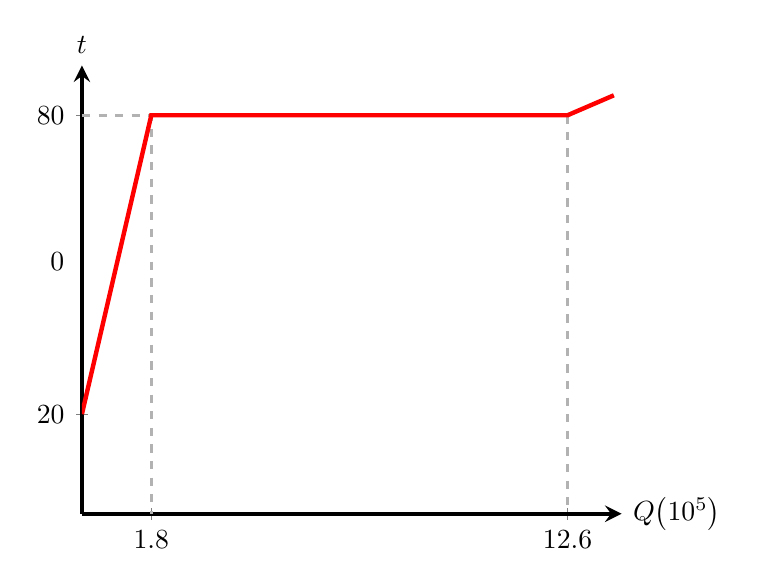
\begin{tikzpicture}  
		\begin{axis}[  ultra thick,
			xmin=0,  
			xmax=14,  
			xtick={1.8,12.6},
			ytick={20,80},
			minor x tick num=0,
			minor y tick num=0,
			ymin=0,  
			ymax=90, 
			samples=300,
			axis lines=center, 
			xlabel=$\xsi{Q}{\left(\xsi{10^5}{\joule}\right)}$, 		ylabel=$\xsi{t}{\celsius}$,
			every axis y label/.style={at=(current axis.above origin),anchor=south},  
			every axis x label/.style={at=(current axis.right of origin),anchor=west},  ]
			\draw [line width=1.0pt,dashed,gray!60!white] (axis cs: 0,80) --(axis cs: 1.8,80)--(axis cs: 1.8,0);
			\draw [line width=1.0pt,dashed,gray!60!white] (axis cs: 12.6,80)--(axis cs: 12.6,0);
			\draw [ultra thick, red] (axis cs: 0,20) --(axis cs: 1.8,80)--(axis cs: 12.6,80)--(axis cs: 13.8,84); 
			
		\end{axis}
		\node[left] at (-0.1,3.2) {0};  
	\end{tikzpicture}
	
\end{center}
	\loigiai{
		Nhiệt lượng chất lỏng thu vào để tăng nhiệt độ từ $\SI{20}{\celsius}$ lên $\SI{80}{\celsius}$:
		$$Q_1=mc\left(t_2-t_1\right).$$
		Nhiệt lượng chất lỏng thu vào để hoá hơi hoàn toàn ở nhiệt độ sôi:
		$$Q_2-Q_1=mL.$$
		Ta có:
		$$\dfrac{Q_2-Q_1}{Q_1}=\dfrac{L}{c\Delta t}\Rightarrow L=\left(\dfrac{Q_2-Q_1}{Q_1}\right)c\Delta t=\left(\dfrac{\SI{12.6}{\joule}-\SI{1.8}{\joule}}{\SI{1.8}{\joule}}\right)\cdot\left[\SI{2500}{\joule/\left(\kilogram\cdot\kelvin\right)}\right]\cdot\left(\SI{80}{\celsius}-\SI{20}{\celsius}\right)=\SI{9E5}{\joule/\kilogram}.$$
	}
\end{ex}
%% ========================================================================
%\begin{ex}
%Thả 1 quả cầu bằng thép có khối lượng $m_1=\SI{2}{\kilogram}$ được nung tới nhiệt độ $\SI{600}{\celsius}$ vào một hỗn hợp nước và đá ở $\SI{0}{\celsius}$. Hỗn hợp có khối lượng tổng cộng là $m_2=\SI{2}{\kilogram}$.
%\begin{enumerate}[label=\alph*)]
%	\item Tính khối lượng nước đá có trong hỗn hợp. Biết nhiệt độ cuối cùng của hỗn hợp là $\SI{50}{\celsius}$.
%	\item Thực ra, trong quá trình trên có một lớp nước tiếp xúc trực tiếp với quả cầu bị hoá thành hơi nên nhiệt độ cuối cùng của hỗn hợp chỉ là $\SI{48}{\celsius}$. Tính khối lượng nước đã hoá thành hơi.
%\end{enumerate}
%Cho:
%\begin{itemize}
%	\item nhiệt dung riêng của thép $c_1=\SI{460}{\joule/\left(\kilogram\cdot\kelvin\right)}$;
%	\item nhiệt dung riêng của nước $c_2=\SI{4200}{\joule/\left(\kilogram\cdot\kelvin\right)}$;
%	\item nhiệt nóng chảy riêng của nước đá $\lambda=\SI{3.4E5}{\joule/\kilogram}$;
%	\item nhiệt hoá hơi riêng của nước $L=\SI{2.3E6}{\joule/\kilogram}$.
%\end{itemize}
%	\loigiai{
%	\begin{enumerate}[label=\alph*)]
%		\item Gọi $m_\text{n}$ và $m_\text{đ}$ lần lượt là khối lượng nước và đá có trong hỗn hợp ban đầu.\\
%		Khi cân bằng nhiệt, tổng nhiệt lượng trao đổi trong hệ bằng 0:
%		$$m_\text{đ}\lambda+m_2c_2\left(t_\text{cb}-0\right)+m_1c_1\left(t_\text{cb}-t_1\right)=0$$
%		$$\Leftrightarrow m_\text{đ}=\dfrac{m_1c_1\left(t_1-t_\text{cb}\right)-m_2c_2t_\text{cb}}{\lambda}=\SI{0.253}{\kilogram}.$$
%		\item Phần nhiệt lượng bị mất mát đi khi chỉ đạt nhiệt độ cân bằng ở $\SI{48}{\celsius}$ thay vì $\SI{50}{\celsius}$ bằng nhiệt lượng $\xsi{m}{\left(\kilogram\right)}$ nước thu vào để tăng nhiệt độ từ $\SI{48}{\celsius}$ lên $\SI{100}{\celsius}$ và hoá hơi hoàn toàn:
%		$$m_2c_2\left(50-48\right)=mc_2\left(100-48\right)+mL\Rightarrow m=\SI{6.67E-3}{\kilogram}=\SI{6.67}{\gram}.$$
%	\end{enumerate}
%	}
%\end{ex}
% ===================================================================
\begin{ex}
	Một bếp dầu đun sôi 1 lít nước đựng trong ấm bằng nhôm khối lượng $m_2=\SI{300}{\gram}$ thì sau thời gian $t_1=\SI{10}{\minute}$ nước sôi. Nếu dùng bếp trên để đun 2 lít nước trong cùng điều kiện thì sau bao lâu nước sôi? Cho nhiệt dung riêng của nước và nhôm lần lượt là $c_1=\SI{4200}{\joule/\left(\kilogram\cdot\kelvin\right)}$, $c_2=\SI{880}{\joule/\left(\kilogram\cdot\kelvin\right)}$. Biết nhiệt do bếp dầu cung cấp một cách đều đặn.
	\loigiai{Vì bếp dầu cung cấp nhiệt lượng một cách đều đặn nên
		$$\dfrac{t_2}{t_1}=\dfrac{\left(m_2c_2+m'_1c_1\right)\Delta t}{\left(m_2c_2+m_1c_1\right)\Delta t}=\dfrac{m_2c_2+m'_1c_1}{m_2c_2+m_1c_1}\Rightarrow t_2\approx\SI{19.4}{\minute}.$$}
\end{ex}
% ===============================================================
\begin{ex}
	Để đúc các vật bằng thép, người ta nấu chảy thép trong lò. Thép ở nhiệt độ \SI{20}{\celsius} được đưa vào lò, hiệu suất của lò là \SI{60}{\percent} (nghĩa là \SI{60}{\percent} nhiệt lượng cung cấp cho lò được dùng vào việc đun nóng thép cho đến khi nóng chảy). Để cung cấp nhiệt lượng, người ta đốt hết \SI{200}{\kilogram} than đá có năng suất tỏa nhiệt là \SI{29e6}{\joule/\kilogram}. Nhiệt nóng chảy riêng của thép là $\lambda=\SI{83.7E3}{\joule/\kilogram}$; nhiệt độ nóng chảy là \SI{1400}{\celsius}; nhiệt dung riêng của thép \SI{460}{\joule/\left(\kilogram\cdot\kelvin\right)}. Xác định khối lượng của mẻ thép đang nấu chảy là bao nhiêu kg (làm tròn kết quả đến chữ số hàng đơn vị)?
	\shortans[oly]{4843}
	\loigiai{
		$m=\SI{4843}{\kilogram}$.
	}
\end{ex}